% ============================================================
\section{Contexto y delimitación del sistema}
% ============================================================

\subsection{Descripción del sistema}

Videojuego de estrategia por turnos desarrollado en C\#, adaptación digital de un juego de mesa inspirado principalmente en Quoridor. Cada jugador mueve su ficha por un tablero hasta alcanzar el extremo contrario, mientras coloca barreras para dificultar el avance del oponente sin bloquear por completo las rutas disponibles.

Está dirigido a personas de 8 años en adelante. El proyecto busca reglas fáciles de aprender, controles accesibles y profundidad estratégica suficiente. Se contempla distribución internacional, por lo que debe soportar varios idiomas (principalmente inglés y español), Unicode, localización de textos, fechas, números y formatos regionales, una interfaz adaptable a palabras de distinta longitud, y almacenamiento en SQL Server.

\begin{center}
  % ============================================================
%  Diagrama de contexto (DFD nivel 0) - "Juego Bastion"
%  Coordenadas en "píxeles" del diagrama original (1261 x 886),
%  con el eje y hacia abajo.
% ============================================================
\definecolor{bordeEntidad}{HTML}{8C7A6B}
\definecolor{fondoEntidad}{HTML}{EFDFD0}
\definecolor{bordeProceso}{HTML}{B5A66E}
\definecolor{fondoProceso}{HTML}{F4E9B4}
\definecolor{lineaFlujo}{HTML}{656D86}
\definecolor{textoDiagrama}{HTML}{404040}

\begin{tikzpicture}[
    x=0.0128cm, y=-0.0128cm,
    font=\fontsize{6.2}{7.5}\selectfont,
    every node/.style={text=textoDiagrama, execute at begin node={\hyphenpenalty=10000}},
    entidad/.style={
      draw=bordeEntidad, line width=0.5pt,
      left color=white, right color=fondoEntidad,
      minimum width=2.30cm, minimum height=1.24cm,
      text width=2.05cm, align=center,
      drop shadow={shadow xshift=1.5pt, shadow yshift=-1.5pt, fill=black!40}},
    proceso/.style={
      circle, draw=bordeProceso, line width=0.5pt,
      left color=white!60!fondoProceso, right color=fondoProceso,
      minimum size=2.10cm, align=center},
    flujo/.style={
      draw=lineaFlujo, line width=0.45pt,
      -{Latex[length=2.4mm, width=1.9mm, fill=lineaFlujo]}},
    etiqueta/.style={fill=white, inner sep=0.8pt},
  ]

  % Marco y pestaña "dfd data"
  \draw[gray!70, line width=0.4pt] (8,8) rectangle (1255,880);
  \draw[gray!70, line width=0.4pt, fill=white]
    (8,8) -- (86,8) -- (86,20) -- (76,30) -- (8,30) -- cycle;
  \node[font=\fontsize{6.2}{7.5}\selectfont\bfseries, anchor=west] at (12,19) {dfd data};

  % Entidades externas y proceso
  \node[entidad] (mod) at (233,111)  {Moderador};
  \node[entidad] (cor) at (1025,111) {Servicio de correo electrónico};
  \node[entidad] (jug) at (138,452)  {Jugador};
  \node[proceso] (sis) at (627,450)  {Juego Bastion};
  \node[entidad] (seg) at (1120,452) {Proveedor del segundo factor};
  \node[entidad] (pla) at (233,792)  {Plataformas de distribución};
  \node[entidad] (sql) at (1025,792) {SQL Server};

  % Flujos: Moderador
  \draw[flujo] (318,160) to[bend right=12] (565,372);
  \draw[flujo] (548,405) to[bend left=12]  (270,160);
  % Flujos: Servicio de correo
  \draw[flujo] (690,372) to[bend right=12] (935,160);
  \draw[flujo] (985,160) to[bend right=12] (708,405);
  % Flujos: Jugador
  \draw[flujo] (228,430) to[bend left=5]   (546,432);
  \draw[flujo] (546,470) to[bend left=5]   (228,474);
  % Flujos: Proveedor del segundo factor
  \draw[flujo] (709,432) to[bend left=5]   (1030,434);
  \draw[flujo] (1030,478) to[bend left=5]  (709,470);
  % Flujos: Plataformas de distribución
  \draw[flujo] (268,745) to[bend left=12]  (546,502);
  \draw[flujo] (566,535) to[bend right=5]  (320,745);
  % Flujos: SQL Server
  \draw[flujo] (709,500) to[bend right=5]  (985,745);
  \draw[flujo] (935,745) to[bend right=12] (690,535);

  % Etiquetas de los flujos
  \node[etiqueta] at (455,243) {Resoluciones de moderación y sanciones};
  \node[etiqueta] at (406,288) {Reportes e historial de chat};
  \node[etiqueta] at (809,243) {Solicitud de correo de verificación};
  \node[etiqueta] at (858,288) {Acuse de entrega o fallo de envío};
  \node[etiqueta] at (382,407) {Jugadas, chat y reportes de conducta};
  \node[etiqueta] at (388,476) {Estado de partida y validación de jugadas};
  \node[etiqueta] at (875,407) {Código de segundo factor a validar};
  \node[etiqueta] at (876,476) {Resultado de la verificación};
  \node[etiqueta] at (405,593) {Actualizaciones y parches distribuidos};
  \node[etiqueta] at (456,638) {Paquete del juego y metadatos de clasificación};
  \node[etiqueta] at (857,593) {Consultas y transacciones SQL};
  \node[etiqueta] at (808,638) {Cuentas, progreso y estado de partidas};
\end{tikzpicture}

  % Para usar la imagen original exportada de Enterprise Architect:
  % 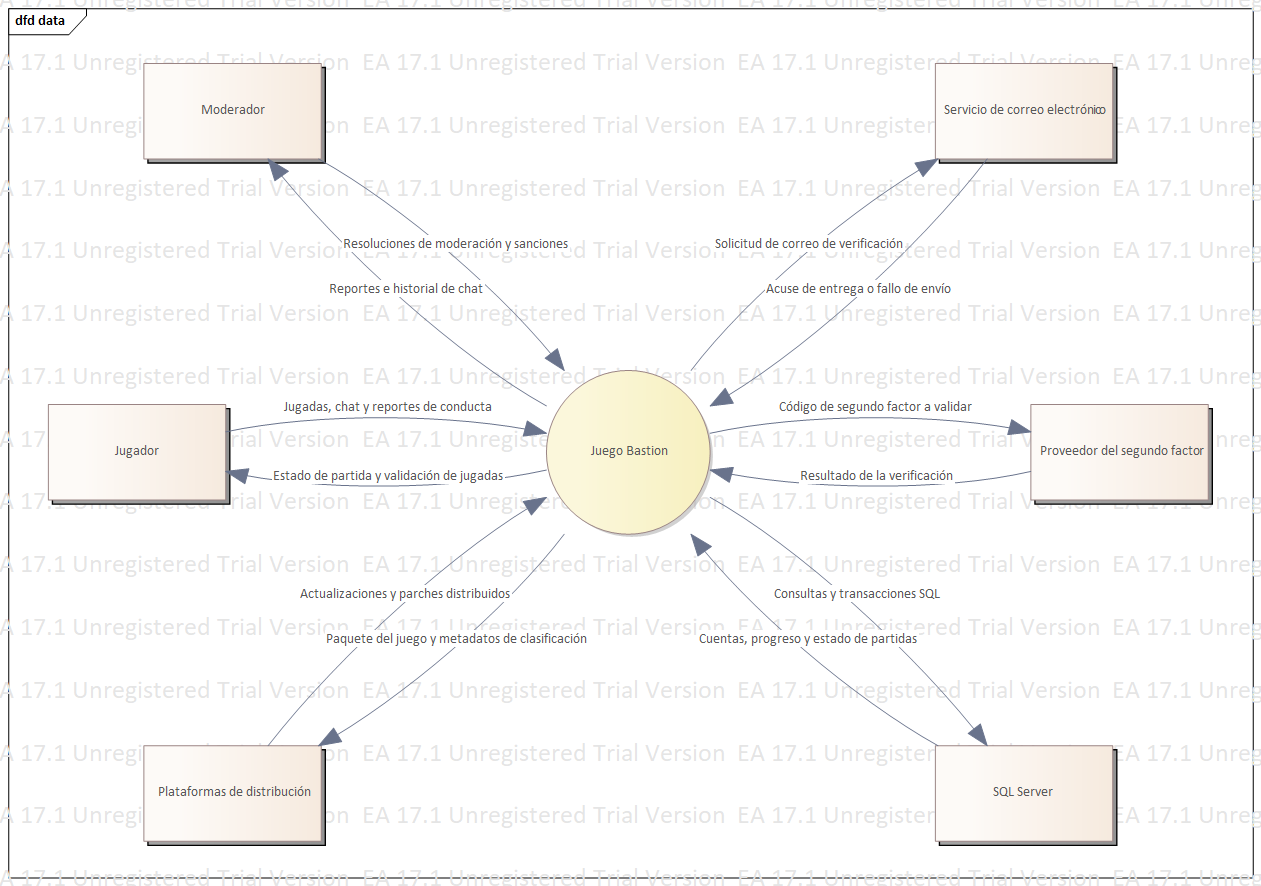
\includegraphics[width=\textwidth]{figuras/diagrama_contexto_original.png}
\end{center}

\subsection{Elementos dentro de la frontera}

\begin{tabla}{|L{4.7cm}|Y|}
\hline
\filacab \cab{Elemento} & \cab{Por qué pertenece al sistema} \\ \hline
\endhead
Cliente de juego (interfaz, tablero, controles, tutorial) &
Es lo que el jugador manipula directamente y lo construye el equipo. \\ \hline
Motor de reglas: movimiento, colocación de barreras y validación de que siempre exista ruta &
Es el núcleo del juego. La validación de “no bloqueo total” obliga a un algoritmo de búsqueda de camino en cada jugada, lo que impacta directamente el presupuesto de respuesta menor a 1 segundo. \\ \hline
Servidor de partidas en línea &
El modo multijugador en línea es un requisito del proyecto y su lógica es responsabilidad del equipo. \\ \hline
Gestión de turnos y estado de partida &
Define quién tiene autoridad sobre el estado y, por tanto, si el servidor actúa como árbitro o como simple retransmisor. \\ \hline
Capa de red sobre TCP &
Debe construirse a la medida porque está prohibido el uso de WebSockets. \\ \hline
Módulo de cuentas: registro, autenticación y segundo factor &
El equipo implementa el flujo completo, aunque se apoye en servicios externos. \\ \hline
Chat de partida y filtro de palabras &
Se desarrolla internamente y condiciona la moderación y la seguridad de los menores. \\ \hline
Módulo de localización &
Atraviesa toda la interfaz y debe diseñarse desde el inicio, no agregarse al final. \\ \hline
Capa de persistencia hacia SQL Server &
El diseño del esquema y de las consultas es responsabilidad del equipo. \\ \hline
\end{tabla}

\subsection{Elementos fuera de la frontera}

\begin{tabla}{|L{3.9cm}|L{5.2cm}|Y|}
\hline
\filacab \cab{Elemento externo} & \cab{Por qué queda fuera} & \cab{Consecuencia arquitectónica} \\ \hline
\endhead
Servicio de correo electrónico & Se consume, no se desarrolla. &
Introduce un tercero en el flujo de cuentas; obliga a manejar fallos y reintentos. \\ \hline
Aplicación autenticadora del segundo factor & Reside en el dispositivo del usuario. &
Solo se implementa el estándar del lado servidor, no la aplicación. \\ \hline
SQL Server (motor) & Producto comercial de terceros. &
Acopla el sistema a su dialecto y a su modelo de disponibilidad. \\ \hline
Infraestructura de servidores y red & Provista externamente. &
La latencia y las caídas del servicio quedan fuera del control del equipo. \\ \hline
Sistema operativo y runtime de .NET & Plataforma base. &
Limita las plataformas en las que puede distribuirse el juego. \\ \hline
Plataformas de distribución & Servicios de terceros. &
Imponen requisitos de contenido y de clasificación por edad. \\ \hline
Quoridor y su propiedad intelectual & Obra de terceros usada como referencia. &
Obliga a reglas, nombres y arte propios. Es una restricción de diseño, no técnica. \\ \hline
Conexión LAN & No está decidida; se evalúa como funcionalidad adicional. &
Mientras no se resuelva Q-02, el extremo de red debe mantenerse configurable para no cerrar la opción. \\ \hline
\end{tabla}
